% siminos/atlas/atlas.tex    pdflatex atlas
% $Author: predrag $ $Date: 2011-11-15 14:06:02 -0500 (Tue, 15 Nov 2011) $
% http://www.cns.gatech.edu/~predrag/papers/Cvit12.pdf

% B&W compile: \draftfalse \colorfigsfalse   in siminos/atlas/setupAtlas.tex
%     then:    pdflatex atlas; bibtex atlas; pdflatex atlas; pdflatex atlas

%\documentclass[referee]{jfm}
\documentclass{jfm}

\newcommand{\version}{atlas ver. 0.1, Dec 10 2011}
% Predrag 					ver. 0.1, Apr 28 2011}

        \input setupAtlas
        \input defAtlas

\title[Charting the state space of turbulent flows]
{Charting the state space of turbulent flows
 in presence of continuous symmetries}

\author[P.\ Cvitanovi{\'c}]
{
P.\ns C\ls V\ls I\ls T\ls A\ls N\ls O\ls V\ls I\ls \'C,
}
\affiliation{
 School of Physics,
 Georgia Institute of Technology,
 Atlanta, GA  30332, USA
}

\pubyear{2012}
%\volume{6??}
%\pagerange{???--???}
%\date{18 December 2011}
%\setcounter{page}{1}
\begin{document}
\maketitle

Symmetry reduction by the `method of slices'
quotients the continuous symmetries of turbulent flows. Within the
symmetry reduced state space, travelling wave solutions reduce to
equilibria, and relative periodic orbits reduce to periodic orbits.
Projections of these solutions and their unstable manifolds from their
$\infty$-dimensional symmetry reduced state space onto suitably chosen 2-
or 3-dimensional subspaces reveal their interrelations and the role they
play in organizing turbulence. Visualizations
of the flow within the slice and its linearization at equilibria enable
us to trace out the unstable manifolds, determine close recurrences,
identify connections between different travelling wave solutions, and
find relative periodic orbits that
are embedded within the chaotic attractor and capture turbulent dynamics.


\section{Introduction}
\label{s:intro}
% former siminos/atlas/intro.tex

The understanding of chaotic dynamics in higher-dimensional systems that
has emerged in the last decade offers a promising dynamical framework to
study turbulence. Here, turbulence is viewed as a walk through a forest
of exact solutions of the governing equations, each solution shaping the
local \statesp\ dynamics.

In this approach, dynamics of moderate \Reynolds\ turbulent flows is
visualized in the $\infty$-dimensional \stateDsp\  using \eqv\ solutions
of the \NSe\ to define dynamically invariant, intrinsic, and
representation independent coordinate frames.
These results inform a new way of thinking about the role {\recurrStr s}
play in shaping turbulence:
The observed {\cohStr s} are the physical images of the flow's
least unstable invariant solutions, with
turbulent dynamics arising from a sequence of transitions between
these states, and
the intrinsic low-dimensionality of turbulence resulting from the low
number of unstable eigendirections for each state.
The unstable \po s are of particular
importance, as they provide the skeleton underpinning the
turbulent dynamics \citep{DasBuch}: the geometry of the \statesp\ flow
near onset of turbulence is shaped by the chaotic saddle, a set of
unstable solutions and their heteroclinic connections.
The long-term goals of this research program are to develop this vision
into quantitative,  predictive description of moderate-{\Reynolds}
turbulence, and to use this description to control flows and explain their statistics.

    \PublicPrivate{}{
In contrast to \pCf, pipe flow has a non-zero mean velocity and cannot
sustain \eqva\ and \po s, so all
unstable invariant solutions are relative, stream-wise travelling
solutions.
    }

Importance of a given invariant solution is made precise by periodic
orbit theory which assigns a deterministic weight with which the solution
contributes to any dynamical average over chaotic component of the flow
\citep{DasBuch}. Consideration of continuous symmetries extends this
theory to sums over \emph{relative} periodic orbits \citep{Cvi07},
time-dependent solutions which recur periodically in co-moving frames
translating and/or rotating along the pipe axis with given stream-wise
and azimuthal velocities, different velocities for each solution.

%%%%%%%%%%%%%%%%%%%%%%%%%%%%%%%%%%%%%%%%%%%%%%%%%
% 2011-10-23 Predrag: replace this Ashley' simulation
%            continuous.tex overheads, and ChaosBook
% TEMPORARY: from siminos/rpo_ks/arxiv-v2/figs, \refref{cont:SCD07})
%
\begin{figure}
\centering
(a)%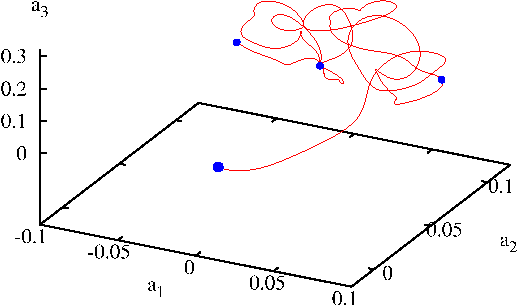
\includegraphics[width=0.45\textwidth,clip=true]{2841GO3a}
~~(b)%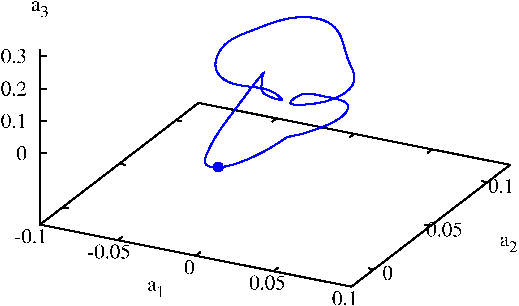
\includegraphics[width=0.45\textwidth,clip=true]{2841GO3b}
  \caption{\label{f:MeanVelocityFrame}
Symmetry reduction $\pS \to \pSRed$ replaces each
(a)
full \statesp\ trajectory $\ssp(\zeit)$ by
(b)
a simpler \reducedsp\ trajectory $\sspRed(\zeit)$, with continuous group
induced drifts quotiented out. Here this is illustrated by the \rpo\
$\RPO{36.92}$ (see \reffig{fig:M1Orb})
(a) %(red)
traced in the full {\statesp} for two $\period{}=36.92$ periods, in the
frame moving with the constant mean axial flow speed $U$ defined in
\refeq{NavStokesDev};
(b) %(blue)
restricted to the symmetry-\reducedsp. Both are projected onto the
$3$\dmn\ frame \refeq{FrenetFrame1}. In the full \statesp\ a \rpo\ traces
out quasi-periodically a highly contorted 2-torus; in the \reducedsp\ it
closes a \po\ in one period $\period{}$.
            }
\end{figure}
%%%%%%%%%%%%%%%%%%%%%%%%%%%%%%%%%%%%%%%%%%%%%%%%%%

In a co-moving frame, moving with the mean phase velocity of a given
solution, a \rpo\ reduces to a \po.
However, as each solution travels with its own mean downstream velocity,
there is no single co-moving frame that can simultaneously reduce
\emph{all} travelling solutions. This problem is here resolved by the
{\mslices} \citep{rowley_reconstruction_2000,BeTh04,SiCvi10,FrCv11}, in
which the group orbit of any full-flow structure is represented by a
single point (see \reffig{fig:BeThTraj}), the group orbit's intersection
with a fixed hypersurface, or the \emph{`\slice'}, analogous to the way a
\PoincSec\ reduces a continuous time orbit to a sequence of points. It
should be noted, however, that a \slice\ is \emph{not} a \PoincSec. A
\slice\ fixes only the group parameters: a continuous time full space
orbit is reduced to a continuous time orbit in the symmetry-\reducedsp,
as in \reffig{f:MeanVelocityFrame}.

Our goals here are two-fold.
(i) We explain what symmetry reduction is, and how with it the geometry
of \statesp\ dynamics is revealed for pipe flow, and
(2) we demonstrate that this new tool enables us to commence a systematic
exploration of the hierarchy of dynamically important invariant solutions
of the pipe flow, starting with two new \rpo s reported here. $3D$
spatial visualization of instantaneous velocity fields,
such as \reffig{fig:N2states}, helps elucidate
the physical processes underlying the formation of unstable coherent
structures. Running concurrently, the $\infty$-dimensional \stateDsp\
representation \citep{GHCW07}, such as \reffig{f:MeanVelocityFrame},
enables us to track the unstable manifolds of invariant
solutions, the heteroclinic connections between them \citep{GHCV08}, and
{provides us with} new insights into the nonlinear \statesp\ geometry and
dynamics of moderate \Reynolds\ wall-bounded flows. Starting in
neighbourhoods of the known \reqva\
 as initial conditions and then searching for
close {recurrences} \citep{pchaot,CviGib10} in the \reducedsp\ yields
educated guesses for locations of \rpo s.

We review  pipe flows, their visualization,
and their symmetries in \refsect{s:review}, where
invariant solutions are classified by their symmetries in
\refappe{appe:DiscSymmPipe}.
The {\mslices}  is described in \refsect{s:slice},
and the computation of invariant solutions and their stability
eigenvalues and eigenvectors in \refsects{s:algorithm}{s:eqbSols}. The
main advances reported in this paper are the symmetry \reducedsp\
visualization and exploration of the moderate-\Reynolds\ turbulent pipe
flow, and determination of new \rpo s\ and their unstable manifolds,
(\refsect{s:rpos}). Outstanding challenges are discussed in
\refsect{s:concl}.

\section{Pipe flows}
\label{s:review}
% former siminos/atlas/review.tex    master file: main.tex

The flow to be considered is that of an incompressible viscous fluid
confined within a pipe of circular cross-section, driven by a pressure
gradient in the axial direction.

In numerical simulations the infinite pipe is represented by periodic boundary
conditions in the stream-wise $z$ direction.

Flow states are typically characterized by the instantaneous kinetic
energy of their deviation from laminar flow, $E = \frac{1}{2}
\Norm{\vec{u}}^2$, and energy dissipation rate $D =
1/\Reynolds\Norm{\bnabla \times \vec{u}}^2$. The dissipation rate is
balanced by the energy fed into the flow as
    \PC{use nomenclature of \cite{SCD07} to describe energy rates}
\beq
\dot{E}=I-D
\,,
\ee{Power=I-D}
where
\(
I =\oint dS \, ({\bf n}\cdot\vec{u})\, p
\)
is the additional instantaneous external power required to maintain
constant flux, over that of the laminar flow.

\subsection{{\StateDsp} visualization of fluid flows}
\label{s:visualStatSp}

As long as one is focusing on a single solution of \NSe, there are many
excellent, physically insightful $3D$ visualizations of the flow:
velocity fields on flow sections, isovorticity surfaces, videos of the
flow, and so on. But today we own dozens of exact \eqv\ and \reqv\
solutions for a given turbulent flow, and we are commencing an exploration of
states of turbulent fluids in terms of the unstable \po\ solutions whose
number, as a function of the increasing period, is growing exponentially.
How are we to visualize \emph{the totality} of these solutions in one go?

The answer was given by \cite{hopf48}, who envisioned the function space
of {\NS} velocity fields as an infinite-dimensional \statesp\ $\pS$ in
which each instantaneous state of $3D$ fluid velocity field $\vec{u}(\bx)$ is
represented as a unique point $\ssp$. In our particular application we
can represent $\ssp = (\vec{u}_{nkm})$ as a vector whose elements are the
primitive discretization variables \refeq{pipeDiscr}. The $3D$ velocity
field given by $\vec{u}_{knm}(\zeit)$, obtained from integration of the
\NSe\ in time, can hence be seen as trajectory $\ssp(\zeit)$ in
$\approx 100,000$ dimensional space spanned by the free variables of our
numerical discretization, with the \NS\ equations \refeq{NavStokesDev}
rewritten as
\beq
   \dot{\ssp} = \vel(\ssp) ,
   \qquad
   \ssp(\zeit) = \ssp(0)
            + \int_0^\zeit \! \mathrm{d}\zeit' \, \vel(\ssp(\zeit'))
\,,
\ee{symbolicNS}
where the current state of the fluid $ \ssp(\zeit)$ is the time-$\zeit$
forward map of the initial fluid state  $\ssp(0)$.

In order to quantify whether two fluid states are close to or far from
each other, one needs a notion of distance between two points in
\statesp, measured here as
\beq
  \Norm{\ssp-\ssp'}^2  = \braket{\ssp-\ssp'}{\ssp-\ssp'} =
\frac{1}{V}
\int_\bCell \! d \bx \;
(\vec{u}-\vec{u}') \cdot (\vec{u}-\vec{u}')
\,.
\ee{innerproduct}
There is no compelling reason to use this {`energy norm'}, other than
that velocity fields is what is given in a numerical computation. What
norm one actually uses depends very much on the application.
Visualizations of trajectory \refeq{symbolicNS} are of necessity
projections onto two or three dimensions. A physically appealing choice
is to monitor the flow in terms of the
symmetry-invariant and physical energy, dissipation and power input
observables $(E(\zeit),D(\zeit),I(\zeit))$, as in
\reffig{fig:M1Orb}\,(b).

For \reqva\ the kinetic
energy is constant and so $D=I$, such solutions sit on the diagonal in
\reffig{fig:M1Orb}\,(b), whereas for relative periodic orbits the kinetic
energy is time-periodic, with $\timeAver{D}=\timeAver{I}$ only for
long-time averages.
    \PC{
    It would be instructive to supplement $(I,E)$, \reffig{fig:M1Orb},
    by the \reffig{fig:M1Orb}\,(b) $(I,D)$  plot as well
    }

While a good check on correctness of numerical data, such projections
bunch all invariant solutions and turbulent flow along the energy-balance
lines, even though the solutions themselves can be (and often are) very
distant from each other.

If two fluid states are clearly separated in
such plot, they are also separated in the high-dimensional \statesp, but
converse is not true; states of very different topology might have
comparable energies, and such plots may obscure some of the most relevant
features of the flow. Furthermore, relations such as \refeq{Power=I-D}
depend on detailed type and geometry of a given problem
\citep{ksgreene88,SCD07}, and further physical observables beyond
$(E(\zeit),D(\zeit),I(\zeit))$ are difficult to construct.
    \PC{add here references to \refeq{Power=I-D} derivations. Does
    Frisch\rf{frisch} do it?}


Recently, \cite{GHCW07} have shown that the dynamics of different regions
of {\statesp}, considered as a high-dimensional vector space,
can be elucidated more profitably by a computationally
straight\-forward sets of \emph{physical} coordinates. One identifies
several prominent states of the flow $\vec{u}_A$, $\vec{u}_B$, $\dots$, such as
{\eqv} states and their linearized stability eigenvectors, states in whose neighborhoods the
turbulent flow spends most of the time, and from them constructs, by
Gram-Schmidt or (anti)-symmetrizations, an orthonormal basis set
$\{\be_1, \be_2, \cdots, \be_n\}$. The evolving fluid state $\bu(\zeit)$
is then projected onto this basis using the inner product
\refeq{innerproduct},
\beq
\ssp(\zeit) =(\ssp_1, \ssp_2, \cdots, \ssp_n, \cdots)(\zeit)
    \,,\qquad
\ssp_n(\zeit) = \braket{\vec{u}(\zeit)}{\be_n}
\,.
\ee{intrSspTraj}
Low-dimensional projections of the flow can be viewed in any of the $2D$ planes
$(\ssp_m, \ssp_n)$ or in $3D$ perspective views $(\ssp_{\ell},\ssp_m,
\ssp_n)$. An example is the \reffig{f:MeanVelocityFrame} projection on
the $3$\dmn\ frame $\{{\be}_1,{\be}_2,{\be}_3\}$ defined in \refeq{FrenetFrame1}.
It is worth emphasizing that the method affords low-dimensional {\em
visualization} without any low-dimensional {\em modeling} or dimension
reduction; the dynamics are computed with fully-resolved direct numerical
simulations. Although the use of particular \reqva\ to define
low-dimensional projections (see \refsect{s:eqbSols}) may appear
arbitrary, the choice turns out to be very useful when the turbulent
flow is chaperoned by a few invariant solutions and their unstable
manifolds, as has been shown in other low Reynolds number settings
\citep{GHCW07}. Such visualizations are a prerequisite to uncovering the
interrelations between (the infinite number of) invariant solutions, and
constructing symbolic dynamics partitions of \statesp\ needed for a
systematic exploration of turbulent dynamics, the key challenge that we
address here for the case of turbulent pipe flows.


\subsection{Symmetries of pipe flow}
\label{s:SymmPipe}
% former siminos/atlas/symm.tex

In many physical applications equations such as \NS\ (in $3D$
representation \refeq{NavStokesDev}, or in the \statesp\ representation
\refeq{symbolicNS}) retain their form under symmetry transformations. On
an infinite domain and in the absence of boundary conditions, the \NSe\
are equivariant under translations, rotations, and
$\bx \to -\bx$, $\bu \to -\bu$ inversion through the origin
\citep{frisch}. In pipe flow the cylindrical wall restricts the rotation
symmetry to rotation about the $z$-axis, and translations along it.

A flow $\dot{\ssp}= \vel(\ssp)$ is said to be $\Group$-\emph{equivariant}
if the form of evolution equations \refeq{symbolicNS} is left invariant
by the set of transformations $\LieEl$ that form the group of symmetries
of the dynamics $\Group$,
\beq
\vel(\ssp)=\LieEl^{-1} \, \vel(\LieEl \, \ssp)
\,,\qquad \mbox{for all } \LieEl \in {\Group}
\,.
\ee{eq:FiniteRot}
Let $\LieEl(\phi,\shift)$ be the shift operator such that $\LieEl(\phi,0)$
denotes an azimuthal rotation by $\phi$ about the pipe axis,
and $\LieEl(0,\shift)$ denotes the stream-wise translation by
$\shift$; let $\sigma$ denote reflection about the $\theta=0$ azimuthal
angle:
%    \PC{2011-10-13: experimenting with APW $\tau \to \LieEl$ renaming}
\bea
\LieEl(\phi,\shift) \, [u,v,w,p](r,\theta,z)
        & = & [u,v,w,p](r,\theta-\phi,z-\shift)
			  \continue
\sigma \, [u,v,w,p](r,\theta,z) \;\; & = & [u,-v,w,p](r,-\theta,z)
\label{pipeSymms}
\eea
%
The \NSe\ for pipe flow are equivariant under these transformations. The
symmetry group of stream-wise periodic pipe flow is thus $\Group =
\On{2}_\theta \times \SOn{2}_z = \Dn{1} \ltimes \SOn{2}_{\theta} \times
\SOn{2}_z$, where $\Dn{1} = \{ e,\, \sigma \}$ denotes azimuthal
reflection, $\ltimes$ stands for a semi-direct product (in general,
reflections and rotations do not commute), and the subscripts $z,\theta$
indicate stream-wise translation and azimuthal rotation respectively. For
an assessment of the discrete symmetries in pipe flow see
\refappe{appe:DiscSymmPipe}.
    \PC{assessment? British obsession...}

While the flow equations are invariant under $\Group$, the state of flow
typically is not. Only the laminar Hagen-Poiseuille \eqv\ is invariant
under all of $\Group$, whereas a generic turbulent state has only the
trivial symmetry group $\{e\}$.

In the literature
(see, \eg\ \cite{ReSaTkYa11}) such \SOn{2} is often referred to as the
circle group $S^1$, also denoted `one-torus' $T^1$.


\subsection{Symmetry-induced coordinate frames}
\label{s:symm}

So far we have not offered any advice as to the choice of basis vectors
in constructing \statesp\ coordinates \refeq{intrSspTraj}. We now show
that at least locally, presence of a continuous symmetry suggests two
natural mutually orthogonal basis vectors, the group action tangent and
curvature vectors.

Consider the one-parameter rotation group \SOn{2} acting on a smooth
periodic function $u(\gSpace + 2\pi) = u(\gSpace)$ defined on domain
$\gSpace \in [0,2\pi)$, expanded in the Fourier basis
\[ %beq
   u(\gSpace) = \sum \ssp_m \mathrm{e}^{\mathrm{i}m\gSpace},
\] %ee{FourierExp1}
where, as $u$ is real, $\ssp_m=\ssp_{-m}^*$. Parametrize the forward
translation by the continuous parameter $\phi$,
\(
    \LieEl(\phi)\,u(\gSpace) = u(\gSpace-\phi)
\,,
\)
or, in the Fourier basis,
\(
   \LieEl(\phi) \,\ssp = \mathrm{diag}\{ \mathrm{e}^{-\mathrm{i}m\phi} \} \,\ssp
\,.
\)
The tangent to the group orbit at the point $\ssp$ is then given by
the first derivative with respect to the group parameter,
The tangent to the group orbit at the point $\ssp$ is then given by
the first derivative with respect to the group parameter,
and the direction of curvature by the second derivative,
\bea
   {\bf t}(\ssp) &=&
   \lim_{\gSpace\to 0}
   \left(\LieEl(\gSpace)\,\ssp - \ssp\right)/\gSpace
   = \mathrm{diag}\{ -\mathrm{i}m \} \, \ssp = \Lg \ssp,
\label{eq:tang}\\
   \kappa(\ssp)\, {\bf n}(\ssp) &=& \Lg^2 \ssp  = - \mathrm{diag}\{m^2\} \, \ssp
   \,,
\label{eq:curv}
\eea
where $\normVec$ is a unit vector normal to the tangent and
$1/\kappa$ is the radius of curvature. The pair of unit vectors
    \PC{2011-10-28
    ``As $\Norm{\LieEl(\gSpace)\slicep}$ is a constant, for the group tangent
    vector $\Lg_\gSpace \slicep$ evaluated at $\slicep$ \refeq{eq:tang}
    %GroupTangField} is normal to $\slicep$, and the term
    $\braket{\slicep}{\Lg_\theta\,\slicep}$ vanishes ($\Lg_{\theta}$ is
    antisymmetric).''
The state vector $\ssp$ is not normal to \normVec(\ssp), as $\braket{\ssp
\Lg^2}{\ssp} = - \Norm{\groupTan(\ssp)}^2 \neq 0$, but can one use it to
produce from $\ssp$ the 3. local eigenbasis unit vector? Have not thought
that through. If we do that here, need to rewrite text leading to
\refeq{PCsectQ0}.
    }
\beq
\{{\be_n},{\be_{n+1}}\} =
\{\groupTan(\ssp)/\Norm{\groupTan(\ssp)},\normVec(\ssp)\}
\ee{FrenetFrame}
forms a local orthogonal Frenet-Serret frame at $\ssp$, and can be useful
in constructing the \statesp\ basis vector set \refeq{intrSspTraj}. For
example, in \reffig{f:MeanVelocityFrame} the \rpo\ $\RPO{36.92}$ is
projected onto the $3$\dmn\ orthogonal frame
\beq
\{{\be}_1,{\be}_2,{\be}_3\}
=
\left\{{\groupTan(\sspRed_0)}/{\Norm{\groupTan(\sspRed_0)}},
\,\normVec(\sspRed_0),\,
(\sspRed_d-\sspRed_0)_{GS} \right\}
\ee{FrenetFrame1}
where $\sspRed_0=\sspRed(0)$ is a point on the \rpo, $\sspRed_d$ is the
most distant point  from $\sspRed_0$ along its symmetry-\reducedsp\ orbit
$\sspRed(\zeit)$, measured in the energy norm \refeq{innerproduct}, and
$(\sspRed_d-\sspRed_0)_{GS}$ is their separation vector, Gram-Schmidt
orthogonalized to $\{\tilde{\be}_1,\tilde{\be}_2\}$.

We note also for later use that, for a time-dependent group parameter
$\gSpace$, the phase speed $\dot{\gSpace}$ along the group tangent
evaluated at the \statesp\ point $\ssp$ (the `Cartan derivative') is
given by
\beq
\LieEl^{-1}\dot{\LieEl} \,\ssp % =e^{-\gSpace \cdot \Lg} \,
     =\mathrm{e}^{-\gSpace \Lg} \,
\left(\frac{\mathrm{d} ~~}{\mathrm{d} \, \zeit} \, % e^{\gSpace \cdot \Lg}\ssp
                             \mathrm{e}^{\gSpace \Lg}\right)\ssp
    =\dot{\gSpace} \, \groupTan(\ssp)
%    =\dot{\gSpace}\cdot \groupTan(\ssp)
\,.
\ee{CartanDer}

\subsection{Relative invariant solutions}
\label{s:RelInvSol}

Along with continuous symmetries come important classes of invariant
solutions referred to as `relative' or `equivariant'
\citep{Huyg1673,Poinc1896}. For pipe flows one expects to find relative
equilibria and \rpo s \citep{Rand82}, associated with the translational
and rotational symmetries of the flow.
These unstable flow-invariant solutions can
only be computed numerically, but they are `exact' in the sense that
they converge to solutions of the \NS\ equations as the
numerical resolution increases.
  \MA{I leave this here pending EVO/skype: ``However, \eqva\ other than
  the laminar state have not been found, and we believe that the symmetry
  under stream-wise shifts precludes any. \NSe\ for pipe are azimuthal
  reflection symmetric, so there are solutions with the azimuthal
  shift~$= 0$, but none other than Hagen-Poiseuille for the stream-wise
  shift~$= 0$, see \refsect{s:symm}. We hence seek spatially
  relative-periodic {\reqvD} and \rpo\ solutions to \refeq{NavStokesDev}
  for the domain $\bCell$.''}


{\em Relative equilibrium} (labeled here $\REQV{}{}$) is a dynamical
orbit whose velocity field \refeq{symbolicNS} lies within the group
tangent space, with a constant phase speed $c$,
% $c=(c_1,\cdots,c_N)$,
and whose time evolution is thus confined to the group orbit,
    \PC{recheck, I might have it normalized wrong; I think it is OK,
        $c$ is angular speed, so $c\,\ssp$ is $\vel$}
    \APW{111027 edited to avoid potential confusion $g(\zeit)$ with $\theta=t$.}
\bea
\vel(\ssp) &=& c \, \groupTan(\ssp) % c \cdot \groupTan(\ssp)
\label{phaseVel}\\
\ssp(\zeit) &=& \LieEl(\gSpace(\zeit)) \, \ssp(0)
%          = \mathrm{e}^{ \zeit  c \Lg} \,  \ssp(0)
%           = \mathrm{e}^{ \zeit\,  c \cdot \Lg} \,  \ssp(0)
\,,\qquad
\ssp(\zeit) \in \pS_{\REQV{}{}}
\nnu
\,.
\eea
While in the case of \SOn{2} symmetry a \reqv\ traces out a loop in the
full \statesp, for a higher-dimensional continuous symmetry it explores
the group orbit $\pS_{\REQV{}{}}$ quasi-periodically, so \reqv\ is
\emph{not} a \po. Rather, as all states in this group orbit are
physically the same state, this is a generalized \eqv\ state. Relative
equilibria can propagate in the stream-wise direction $z$ (travelling
waves), in azimuthal $\theta$ direction (rotational waves), or both. As
noted in \refsect{s:intro}, for pipe flows many stream-wise travelling
\reqva\ have been discovered, satisfying \refeq{phaseVel}
\beq
   \LieEl(0,-ct)\,\vec{u}(\zeit) - \vec{u}(0) = \vec{0}
\,,
\ee{pipeAxTW}
where $c$ is the stream-wise phase speed.

A {\rpo} $p$ is an orbit in {\statesp} $\pS$ which exactly recurs
\[ %beq
\ssp(\zeit) = \LieEl_p \, \ssp(\zeit + \period{p} )
    \,,\qquad
\ssp(\zeit) \in \pS_p
\] %ee{RPOrelper1}
after a fixed {relative period} $\period{}$, but shifted by a fixed group
action ${\LieEl}$ that maps the endpoint $\ssp (\period{} ) $ back
into the initial point cycle point $\ssp (0) $.
In the pipe flow cylindrical coordinate system
a \rpo\ is a time-dependent velocity field
\beq
\bu_p(r,\theta,z,t)=\bu_p(r,\theta+\phi_p,z+ \shift_p,t+\period{p})
\ee{RPOpipe}
that recurs after time $\period{p}$, rotated and shifted by $\phi_p$ and
$\shift_p$.
In our Newton search for a \rpo\ $p$, we seek the zeros of
\beq
   \vec{f}(\vec{u}(0),\period{},\shift)
\,=\, \LieEl(0,-\shift)\,\vec{u}(\period{}) - \vec{u}(0) \,=\, \vec{0}
\,,
\ee{eq:fRPO}
for some $\vec{u}_p$ with period $\period{p}$ and shift $\shift_p$.

Continuous symmetry parameters (`phases' or `shifts')
$\{\gSpace_j\}=\{\phi_p,\shift_p\}$
% $\{\gSpace_1,\cdots,\gSpace_N\}$
are real numbers, ratios $\pi/\gSpace_j$ are almost never rational, and
\rpo s are almost never eventually periodic; for pipe the time evolution
of a relative periodic point thus sweeps out quasi-periodically the
$3$\dmn\ group orbit $\pS_p$ without ever closing into a \po, unless the
dynamics is restricted to a discrete-symmetry invariant subspace.



\section{Reduction of continuous symmetry}
\label{s:slice}
% former siminos/atlas/slice.tex
% Predrag 2011-08-11: transfered here text from
% talks/predrag/continuous/continuous.tex
% as the outline of the section

We have seen that in presence of the continuous $\SOn{2}$ symmetry
\reqva\ and \rpo s are 2- and 3-dimensional manifolds of physically
equivalent states. How are we to compare a pair of such states? We shall
do this here by determining the minimal distance between them.

The \emph{group orbit} $\pS_\ssp $ of a \statesp\ point $\ssp \in \pS$ is
traced out by the set of all group actions
\beq
\pS_\ssp = \{\LieEl\,\ssp \mid \LieEl \in {\Group}\}
% \,,\qquad \pS_\ssp \subset \pS
\,.
\ee{sspOrbit}
Any state in the  group orbit set $\pS_{\ssp}$
is physically equivalent to any other. The action of a symmetry group
thus foliates the \statesp\ into a union of group orbits,
\reffig{fig:BeThTraj}\,(a).

%%%%%%%%%%%%%%%%%%%%%%%%%%%%%%%%%%%%%%%%%%%%%%%%%
% 2011-08-23 Predrag: replaces BeThTraj.pdf from
% dasbuch/book/FigSrc/inkscape/BeThTraj.svg
% 2011-09-09 Predrag: updated
%            continuous.tex overheads, and ChaosBook
\begin{figure}
 \begin{center}
  \setlength{\unitlength}{0.40\textwidth}
  %% \unitlength = units used in the Picture Environment
(a)~~
  \begin{picture}(1,1.07471658)%
    \put(0,0){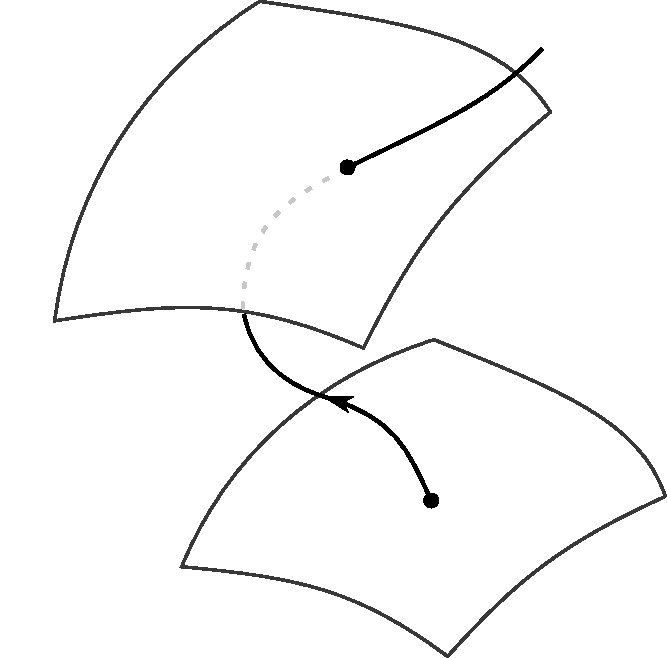
\includegraphics[width=\unitlength]{BeThTrajTeX}}%
    \put(0.28879298,1.02196543){\color[rgb]{0,0,0}\rotatebox{-22.37140782}{\makebox(0,0)[lb]{\smash{$\pS_{\ssp(\zeit)}$}}}}%
    \put(0.55566402,0.45078735){\color[rgb]{0,0,0}\rotatebox{-16.6673442}{\makebox(0,0)[lb]{\smash{$\pS_{\ssp(0)}$}}}}%
    \put(0.63028127,0.18433597){\color[rgb]{0,0,0}\rotatebox{0.03136739}{\makebox(0,0)[lb]{\smash{$\ssp(0)$}}}}%
    \put(0.46253394,0.70182304){\color[rgb]{0,0,0}\rotatebox{0.03136739}{\makebox(0,0)[lb]{\smash{$\ssp(\zeit)$}}}}%
    \put(0.03852492,0.09250899){\color[rgb]{0,0,0}\rotatebox{0.11031334}{\makebox(0,0)[lb]{\smash{$\pS$}}}}%
  \end{picture}%
~~(b)
  \begin{picture}(1,1.07315413)%
    \put(0,0){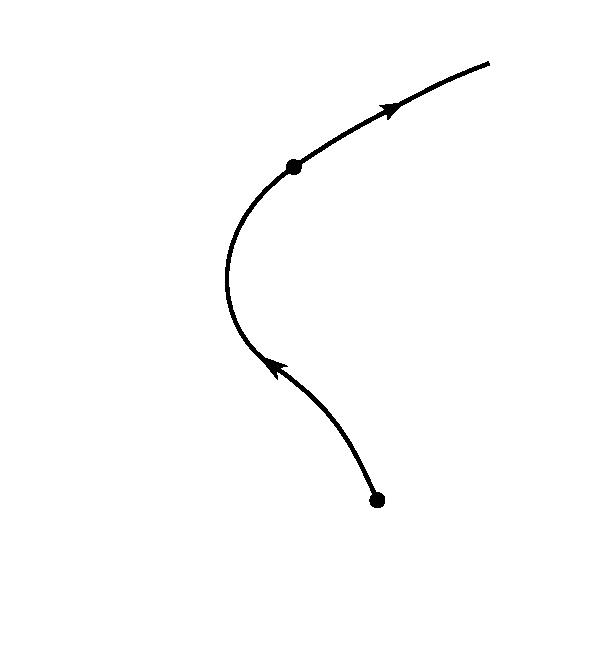
\includegraphics[width=\unitlength]{BeThRedTeX}}%
    \put(0.19912369,0.17144733){\color[rgb]{0,0,0}\rotatebox{0.11031334}{\makebox(0,0)[lb]{\smash{$\pSRed$}}}}%
    \put(0.63028127,0.18433598){\color[rgb]{0,0,0}\rotatebox{0.03136739}{\makebox(0,0)[lb]{\smash{$\sspRed(0)$}}}}%
    \put(0.46253394,0.70182305){\color[rgb]{0,0,0}\rotatebox{0.03136739}{\makebox(0,0)[lb]{\smash{$\sspRed(\zeit)$}}}}%
  \end{picture}%
 \end{center}
% (a) 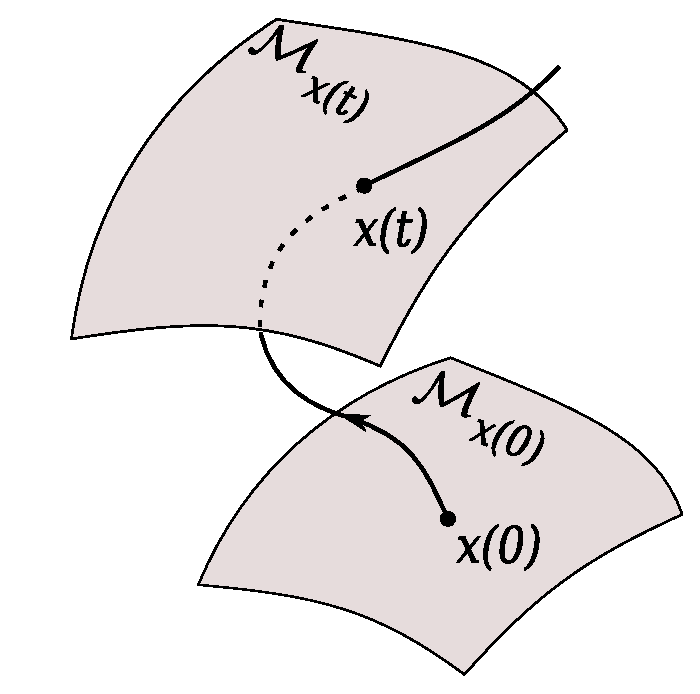
\includegraphics[width=0.45\textwidth]{BeThTraj}
  \caption{\label{fig:BeThTraj}
(a)
The group orbit $\pS_{\ssp(0)}$ of \statesp\ point $\ssp(0)$, and the
group orbit $\pS_{\ssp(\zeit)}$ reached by the trajectory $\ssp(\zeit)$ time $t$
later.
(b)
Symmetry reduction $\pS \to \pSRed$ replaces each full \statesp\
group orbit $\pS_{\ssp}\subset\pS$ by a single point $\sspRed \in \pSRed$.
  }
\end{figure}
%%%%%%%%%%%%%%%%%%%%%%%%%%%%%%%%%%%%%%%%%%%%%%%%%%

For the example at hand, a pipe flow (or a \pCf) with two periodic
boundary conditions, the symmetry group $\Gpipe$ contains two commuting
\SOn{2} rotations. Each \SOn{2} subgroup group orbit is (topologically) a
circle, see \reffig{fig:2840GOt135th0}, and together they sweep out a
$T^2$ torus, see \reffig{fig:2830GO6}.
    \PC{we should have a look at \reffig{fig:2830GO6} projected onto
    the same coordinate frame as \reffig{fig:M1FULL}, as well.
        {\bf APW} 111111 I think fig 19 in flotsam uses fig 9 coords.
        Needs axis scaling corrected; can dig it out, but too many
        plots already?
         {\bf PC} two edits later all figures are renumbered, so who know
        what was `fig 19'? Use their labels.
    }
    \PC{What happens if you plot \reffig{fig:2840GOt135th0}\,(b) and
    \reffig{fig:2830GO6}\,(b) in the same $\ssp'=\ssp_\mathrm{N2\_LB}$ frame as
    \reffig{fig:2840GOt135th0}\,(a)? We would like to illustrate that
    turbulent states is much more contorted, would be nice if we could
    plot them in the same frame?
        {\bf APW} 111111 To get fig (b) with inflexion I had to run
        slicing until got a jump, hence frame with $\ssp'=\ssp_\mathrm{N2\_LB}$.
        Also gives a case where $\ssp$ is `not so close' to $\ssp'$.
    }
\begin{figure}
  \centering
(a)%\includegraphics[width=0.45\textwidth]{2839GOLBth0}
(b)%\includegraphics[width=0.45\textwidth]{2840GOt135th0}
  \caption{\label{fig:2840GOt135th0}
    %\label{fig:M1groupOrb}
Projections of group orbits of two states $\ssp$ (in $\approx
100,000$-dimensional {\statesp}) onto a stationary Frenet-Serret frame
given by unit vectors in the directions
$\{\groupTan_z(\ssp'),\groupTan_\theta(\ssp'),\normVec_z(\ssp')\}$ (see
\refeq{FrenetFrame}). The group orbit is generated by
$\LieEl(0,\shift)\,\ssp$, i.e. by axial shifts, and plotted relative to the
point $\ssp'$.
In (a) $\ssp=\ssp'=\ssp_\mathrm{N2\_LB}$, being a ``lower-branch'' \reqv\
described in \refsect{s:eqbSols};
in (b) $\ssp$ is a strongly nonlinear turbulent state
and $\ssp'=\ssp_\mathrm{N2\_M1}$.
Group orbits are only topologically circles, and inflections are possible
when $\ssp$ is not so close to $\ssp'$.
%{APW 111027 For N2_UB, only see mild distortions;
% see fig 15(b) of dailyBlog}
  }
\end{figure}


\begin{figure}
  \centering
(a)%\includegraphics[width=0.45\textwidth]{2839GOLB}
(b)%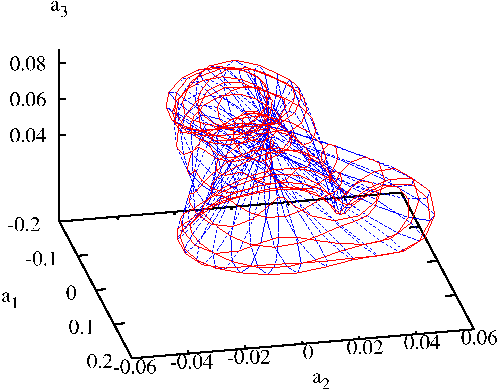
\includegraphics[width=0.45\textwidth]{2840GOt135M1}
  \caption{\label{fig:2830GO6}
    %\label{fig:M1groupOrb}
As \reffig{fig:2840GOt135th0}, but with the
full 2\dmn\ $\SOn{2}_{\theta} \times \SOn{2}_z$ group orbits traced out
by shifts in both $z$ and $\theta$. Loops in solid red correspond to
shifts in $z$, dashed blue loops to shifts in $\theta$.
%(a) \Reqv\ N2\_LB, (b) \Reqv\ N2\_UB.
  }
\end{figure}

The goal of \emph{symmetry reduction} is to replace each group orbit by a
unique point in a lower-dimensional symmetry-\reducedsp\ $\pSRed =
\pS/\Group$, as sketched in \reffig{fig:BeThTraj}. Several symmetry
reduction schemes are reviewed in \refref{SiCvi10}. Here we shall
describe the \mslices\ \citep{rowley_reconstruction_2000,BeTh04,FrCv11}, the
only method that we find practical for a symmetry reduction of
turbulent solutions of highly nonlinear flows, see \refsect{s:rpos}.

In the \mslices\ the symmetry reduction is achieved by cutting the group
orbits with a finite set of hyperplanes, one for each continuous group
parameter, with each group orbit of
symmetry-equivalent points represented by a single point, its
intersection with the \slice.
The procedure is akin to (but distinct from)
cutting across continuous-time parametrized trajectories by
means of Poincar\'e sections.
As is the case for Poincar\'e sections,
choosing a `good' \slice\ is a dark art. Our guiding principle is to chose
a \slice\ such that the distance between a `{\template}' state {\slicep} and nearby
group orbits is \emph{minimized}, \ie, identify the point $\sspRed$ on the group
orbit \refeq{sspOrbit} of a nearby state $\ssp$ which is the closest
match to the {\template} point {\slicep}.


\subsection{\Mslices; a local chart}

After some experimentation and observations of turbulence in a given
flow, one can identify a set of dynamically important unstable
{\recurrStr s}.  For example, coherent streaky structures have been
observed in pipe flow where `very large scale motions' have
length scales comparable to the pipe radius.

We shall refer to this catalogue of $m$ representative snapshots
or `reference states', either precomputed or
experimentally measured, as  \emph{\template s}
\citep{rowley_reconstruction_2000}, each an instantaneous state of the
$3D$ fluid flow represented by a
\emph{point} $\slicep{}^{(j)}$, $j=1,2,\cdots,m$, in the
\statesp\ $\pS$ of the system. The symmetries of the flow (i.e.\ the
$\LieEl\in\Group$) are then used to shift and rotate the {\template}
$\slicep$ until it overlies, as well as possible, the {\cohStr} of
interest $\ssp$, by minimising the distance
\beq
\Norm{\ssp - \LieEl(\gSpace)\,\slicep}
%    = \Norm{\LieEl(-\gSpace)\,\ssp - \slicep}
%    = \Norm{\sspRed - \slicep}
\, .
\ee{minDistance}
The entire group orbit of $\ssp$ is then replaced
by the closest match to
the template pattern,
given by
$\sspRed=\LieEl^{-1}\ssp$, %=\LieEl(-\gSpace)\ssp$,
as shifting does not affect the norm,
$\Norm{\ssp-\LieEl\,\slicep}=\Norm{\sspRed-\slicep}$.
The symmetry \reducedsp\ $\pSRed$, of dimension $(d\!-\!1)$, consists of
the set of closest matches $\sspRed$, one element for each full \statesp\ $\pS$
group orbit; the bar on $\sspRed$
indicates the unique point on the group orbit of $\ssp$ closest to
the \template\ \slicep.

For the reduction of the azimuthal
$\SOn{2}_\theta$ symmetry (and likewise for the stream-wise translations
$\SOn{2}_z$ symmetry), the minimal distance satisfies the extremum
condition
\[
\frac{\partial}{\partial \gSpace} \Norm{\ssp - \LieEl(\gSpace)\,\slicep}^2
   =
2\, \braket{\ssp - \LieEl\,\slicep}{\Lg_\gSpace \,\LieEl\,\slicep}
   =
2\, \braket{\sspRed - \slicep}{\Lg_\gSpace \slicep}
   = 0
    \, ,
\]
given that group orbits are smooth differentiable manifolds.
As $\Norm{\LieEl(\gSpace)\slicep}$ is a constant,
the group tangent vector $\Lg_\gSpace \slicep$
evaluated at $\slicep$
\refeq{eq:tang} %GroupTangField}
is normal to $\slicep$, and
the term $\braket{\slicep}{\Lg_\theta\,\slicep}$ vanishes
($\Lg_{\theta}$ is antisymmetric).
Therefore the point $\sspRed$ on the group
orbit that lands in the \slice, satisfies the \emph{\slice\ condition}
\beq
\braket{\sspRed}{\sliceTan{\theta}} = 0
    \,,\quad
\sliceTan{\theta} = \Lg_\theta \slicep
    \,.
\ee{PCsectQ0}
The \slice\ so defined is therefore
a hyperplane that includes the origin,
normal to the \template\ group tangent %$\sliceTan{\theta}$
evaluated at the \template.

%%%%%%%%%%%%%%%%%%%%%%%%%%%%%%%%%%%%%%%%%%%%%%%%%%%%%%%%%%%%%%%%
%% slice.*, inflectHype.*: see dasbuch/book/FigSrc/inkscape/00ReadMe.txt
%% rpo.* hand-drawn in dasbuch/book/FigSrc/xfig/rpo.fig
%% xfig exported -> FigSrc/inkscape/rpo.fig
%% inkscape exported -> rpo.eps + LaTeX, hand edited in the macros
%% Predrag 2011-08-27 replaced rpo.pdf by rpoSlice.pdf
%% remember to insert rpoSlice.pdf into ChaosBook

 \begin{figure}
 \begin{center}
  \setlength{\unitlength}{0.40\textwidth}
  %% \unitlength = units used in the Picture Environment
(a)
  \begin{picture}(1,0.87085079)%
    \put(0,0){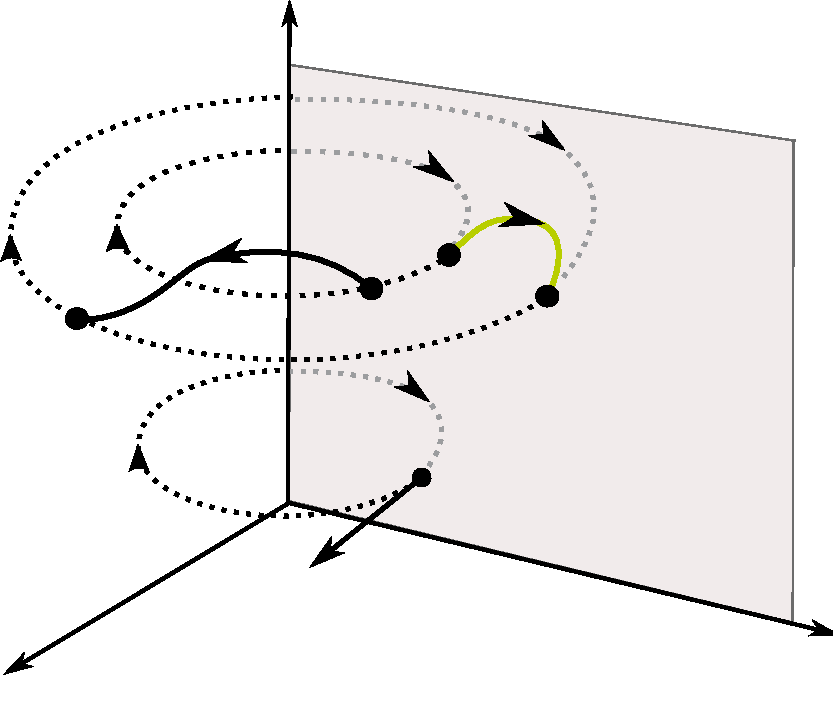
\includegraphics[width=\unitlength]{slice}}%
    \put(0.82835155,0.19007659){\color[rgb]{0,0,0}\rotatebox{-14.84025424}{\makebox(0,0)[lb]{\smash{$\pSRed$}}}}%
    \put(0.07077338,0.28688228){\color[rgb]{0,0,0}\rotatebox{0.0313674}{\makebox(0,0)[lb]{\smash{$\LieEl\,\slicep$}}}}%
    \put(0.53023327,0.26593335){\color[rgb]{0,0,0}\rotatebox{0.0313674}{\makebox(0,0)[lb]{\smash{$\slicep$}}}}%
    \put(0.4284954,0.179285){\color[rgb]{0,0,0}\rotatebox{0.0313674}{\makebox(0,0)[lb]{\smash{$\sliceTan{}$}}}}%
    \put(0.00798985,0.42305068){\color[rgb]{0,0,0}\rotatebox{0.0313674}{\makebox(0,0)[lb]{\smash{$\ssp(\zeit)$}}}}%
    \put(0.65766235,0.45412105){\color[rgb]{0,0,0}\rotatebox{0.0313674}{\makebox(0,0)[lb]{\smash{$\sspRed(\zeit)$}}}}%
    \put(0.06916446,0.74280851){\color[rgb]{0,0,0}\rotatebox{0.0313674}{\makebox(0,0)[lb]{\smash{$\LieEl(\zeit)$}}}}%
  \end{picture}%
~~~
%(b)
%  \begin{picture}(1,0.76829268)%
%    \put(0,0){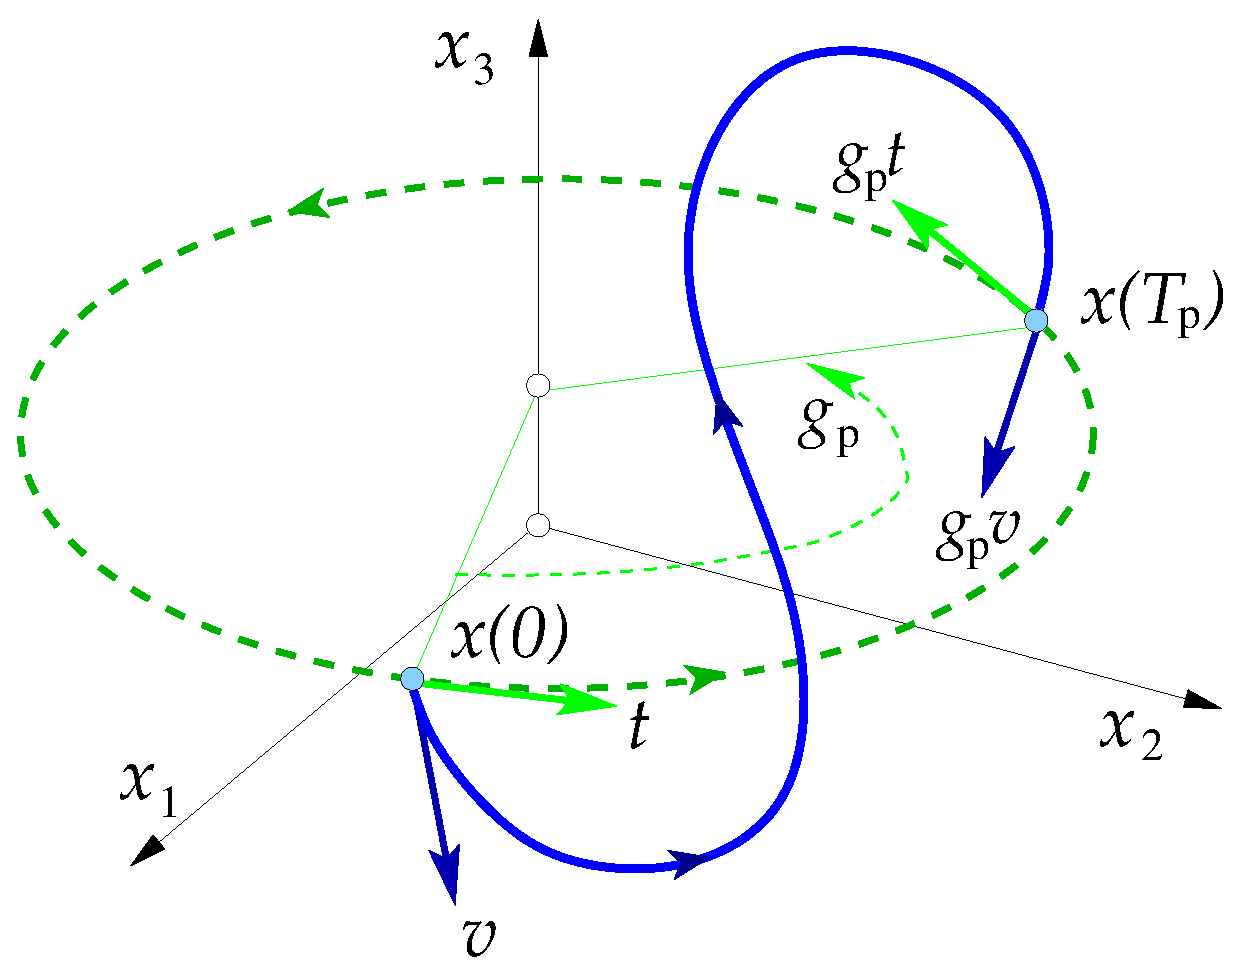
\includegraphics[width=\unitlength]{rpo}}%
%    \put(0.08347773,0.13075729){\color[rgb]{0,0,0}\makebox(0,0)[lb]{\smash{$\ssp_1$}}}%
%    \put(0.63887473,0.43082864){\color[rgb]{0,0,0}\makebox(0,0)[lb]{\smash{$\LieEl_p$}}}%
%    \put(0.86678218,0.51919883){\color[rgb]{0,0,0}\makebox(0,0)[lb]{\smash{$\ssp(\period{p})$}}}%
%    \put(0.88288656,0.17407601){\color[rgb]{0,0,0}\makebox(0,0)[lb]{\smash{$\ssp_2$}}}%
%    \put(0.66771991,0.63957392){\color[rgb]{0,0,0}\makebox(0,0)[lb]{\smash{$\LieEl_p \groupTan$}}}%
%    \put(0.75119764,0.33940065){\color[rgb]{0,0,0}\makebox(0,0)[lb]{\smash{$\LieEl_p \vel$}}}%
%    \put(0.35317501,0.24623991){\color[rgb]{0,0,0}\makebox(0,0)[lb]{\smash{$\ssp(0)$}}}%
%    \put(0.34033228,0.72784219){\color[rgb]{0,0,0}\makebox(0,0)[lb]{\smash{$\ssp_3$}}}%
%    \put(0.49760473,0.17244519){\color[rgb]{0,0,0}\makebox(0,0)[lb]{\smash{$\groupTan$}}}%
%    \put(0.36275609,0.00233001){\color[rgb]{0,0,0}\makebox(0,0)[lb]{\smash{$\vel$}}}%
%  \end{picture}%
%~~~
%\\
(b)
  \begin{picture}(1,0.87085079)%
    \put(0,0){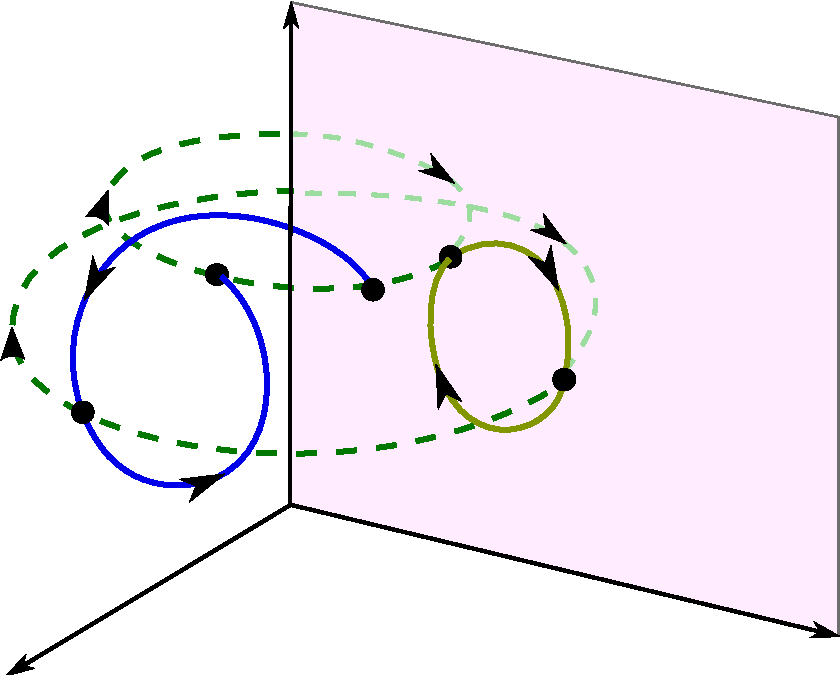
\includegraphics[width=\unitlength]{rpoSlice}}%
    \put(0.82835153,0.19007656){\color[rgb]{0,0,0}\rotatebox{-14.84025432}{\makebox(0,0)[lb]{$\pSRed$}}}%
    \put(0.40925459,0.45713857){\color[rgb]{0,0,0}\rotatebox{0.0313674}{\makebox(0,0)[lb]{\smash{$\ssp(0)$}}}}%
    \put(0.71354118,0.39765314){\color[rgb]{0,0,0}\rotatebox{0.0313674}{\makebox(0,0)[lb]{\smash{$\sspRed(\zeit)$}}}}%
    \put(0.13171187,0.38813817){\color[rgb]{0,0,0}\rotatebox{0.0313674}{\makebox(0,0)[lb]{\smash{$\LieEl(\zeit)$}}}}%
    \put(0.02168739,0.31359574){\color[rgb]{0,0,0}\rotatebox{0.0313674}{\makebox(0,0)[lb]{\smash{$\ssp(\zeit)$}}}}%
    \put(0.15576193,0.48769256){\color[rgb]{0,0,0}\rotatebox{0.0313674}{\makebox(0,0)[lb]{\smash{$\ssp(\period{})$}}}}%
    \put(0.54113911,0.50476963){\color[rgb]{0,0,0}\rotatebox{0.0313674}{\makebox(0,0)[lb]{\smash{$\sspRed(0)$}}}}%
  \end{picture}%
 \end{center}
 \caption{\label{fig:slice}
The \mslices, a \statesp\ visualization:
(a)
\Slice\ $\pSRed \supset \pS/\Group$ lies in the $(d\!-\!N)$\dmn\
hyperplane \refeq{PCsectQ0} normal to $\sliceTan{}$, where $\sliceTan{j}$
span the  $N$\dmn\ space tangent to the group orbit $\LieEl\,\slicep$
(dotted line) evaluated at the {\template} point $\slicep$. The
hyperplane intersects {\em all} full \statesp\ group orbits (green
dashes). The full \statesp\ trajectory $\ssp(\zeit)$ (blue) and the
\reducedsp\ trajectory $\sspRed(\zeit)$ (green) are equivalent up to a
`moving frame' rotation $\ssp(\zeit)=\LieEl(\zeit)\,\sspRed(\zeit)$, where
$\LieEl(\zeit)$ is a shorthand for $\LieEl(\gSpace(\zeit))$.
(b)
In the full \statesp\ $\pS$ a \rpo\ $\ssp(0) \to \ssp(\zeit) \to
\ssp(\period{})$ returns to the group orbit of $\ssp(0)$ after time
$\period{}$ and a rotation by $\LieEl$,  $\ssp(0)=\LieEl \, \ssp
(\period{})$. For flows with continuous symmetry a generic \rpo\ fills
out quasi-\-periodically what is topologically a torus. In the \slice\
$\pSRed$ the symmetry-reduced orbit is periodic, $\sspRed(0) =
\sspRed(\period{})$. This is a highly idealized sketch: A group orbit is
a $N$\dmn\ manifold, and even for $\SOn{2}$ it is usually only
topologically a circle (see \reffig{fig:2840GOt135th0}), and can
intersect a hyperplane any number of times  (see \reffig{fig:sliceimage}).
 }
 \end{figure}

When $\ssp$ is varies in time, $\dot{\ssp}=\vel(\ssp)$,
the template $\slicep$ tracks the motion
using the slice condition \refeq{PCsectQ0} to
minimise $\Norm{\ssp(\zeit)-\LieEl(\theta(\zeit))\slicep}$,
and the
full-space trajectory $\ssp(\zeit)$ is thus rotated into the {\reducedsp},
$\sspRed(\zeit) = \LieEl^{-1}\,\ssp(\zeit)$,
by appropriate
\emph{moving frame} angles $\{\gSpace(\zeit)\}$, as depicted in
\reffig{fig:slice}\,(a).
%
Specializing to $\SOn{2}$, one can write the
equations for the \reducedsp\
flow, $\sspRed(\zeit) \in \pSRed$,
confined to the \slice, $\dot{\sspRed} = \velRed(\sspRed)$,
as
\bea
\velRed(\sspRed) &=& \vel(\sspRed)
     \,-\, \dot{\gSpace}(\sspRed) \, \groupTan(\sspRed)
\label{EqMotMFrame}\\
\dot{\gSpace}(\sspRed) &=& \braket{\vel(\sspRed)}{\sliceTan{}}
                       /\braket{\groupTan(\sspRed)}{\sliceTan{}}
\,.
\label{reconstrEq}
\eea
In other words, $\vel$, the velocity in the full \statesp, can be written
as the sum of $\velRed$, the velocity component in the \slice, and
$\dot{\gSpace}\,\groupTan$, the Cartan derivative \refeq{CartanDer} or
the velocity component within the group tangent space. The
$\dot{\gSpace}$ equation is the {\em reconstruction equation}: its
integral keeps track of the group shifts in the full \statesp. In
particular, if  \sspRed\ is a point on a \reqv\ \refeq{phaseVel}, the full \statesp\
velocity equals the phase velocity, and $\velRed(\sspRed) = 0$, \ie,
\reqva\ are always reduced to \eqva\ in the \reducedsp. It should be
emphasized that we never integrate the reduced equations
\refeq{EqMotMFrame}; numerical simulations are always carried out in the
full \statesp. Slicing is implemented as postprocessing of numerical or
experimental data, by rotating full \statesp\ trajectories into the
\slice, as in \reffig{fig:sliceimage}.

The \mslices\ as implemented here associates a `\slice' hyperplane to each
\template. As the inertial manifold is a highly contorted, nonlinear
curved manifold embedded in the $\infty$-dimensional \statesp, any such
linearization is good only locally: a single template cannot be a good
match  globally.
    %
%  \includegraphics[width=1.00\textwidth,clip=true]{slicePhil0}


\subsection{Charting the \reducedsp}
\label{s:chartingslice}

\APW{111104 The first sentence requires simplifying!}
As group orbits % of compact Lie groups
are smooth manifolds (in case at hand, 2-tori), have natural linear
representations (under linear action of a symmetry group, \statesp\
decomposes into a sum over irreducible subspaces), and have natural local
coordinate frames (the group tangent, curvature Frenet-Serret frames
\refeq{FrenetFrame}), good \slice s should be easier to construct than
the elusive ``good'' Poincar\'e sections of the time-evolution flows.
Indeed, as a generic \slice\ \refeq{PCsectQ0} is the set of all
group-orbit points closest to a given template, it slices the group
orbits of \emph{all} full \statesp\ points \citep{FrCv11}. However, for a
nonlinear flow, there is no single \slice\ that really does the job: our
\slice\ is locally a hyperplane, expected to be a good description of
solutions similar to a given template in some open neighborhood. The
variational distance condition \refeq{PCsectQ0} is only an extremum
condition, and as the group orbits of highly nonlinear states are highly
contorted (see \reffig{fig:2830GO6}\,(b)), they can have many
extrema, and multiple sections by a \slice\ hyperplane. For example, an
\rpo\  torus is always intersected by a \slice\ hyperplane in two or more
sections, see \reffig{fig:sliceimage}.
    \PC{\refFig{fig:sliceimage}, new proposal: take points on the good,
    blue \po, run each along the group orbit until $\sspRSing \in S$
    where it intersects the \sset, see \refeq{sspRSing}, and thus plot
    the border of where the local slice ends, once on the left, and once
    on the right of the template. Catch - I have not thought this
    through, not sure that the condition \refeq{sspRSing} can be
    satisfied on every group orbit...
    }
    \PC{\refFig{fig:sliceimage}: Eventually most of my caption will go
    into the text proper. I guess we are lucky with this \rpo\ but it
    does not illustrate the problem well - generically there can be many
    \po\ slice cuts of the same \rpo. [please read Predrag and Ashley's
    blog entries of {\bf [2011-10-28]}.
    }
    \PC{It's safer to move figures into flotsom.tex than to just erase
    them, both for broken links and for future reference. My initial
    \reffig{ks22rpo16mf} illustrates the point, but I had work to recover
    it. For example, the slice cuts need not be `separate.'}

%%%%%%%%%%%%%%%%%%%%%%%%%%%%%%%%%%%%%%%%%%%%%%%%%%%%%%%%%%%%%%%%%%%%%
\begin{figure}
   \centering
   %\includegraphics[width=0.45\textwidth]{2841GO3S}
   \caption{\label{fig:sliceimage}
      Every slice hyperplane cuts every group orbit at least twice (see
      \reffig{fig:slice}), once at       orbit's closest passage to the
      template, with positive curvature \refeq{eq:curv},   and another
      time at the most distant passage, also satisfying the slice
      condition \refeq{eq:slcond}, but with negative curvature. An
      $\SOn{2}$ \rpo\ is topologically a torus, so the two cuts are the
      two \po\ images of the same \rpo, the good close one, and the bad
      distant one, on the other side of {\sset}, and thus not in the
      slice. Here this is illustrated by close cut (blue) of the \rpo\
      $\RPO{36.92}$ torus, \reffig{f:MeanVelocityFrame}\,({\it b}),
      plotted together with the most distant cut (red), in the same slice
      hyperplane, but not in the slice.
   }
\end{figure}
%%%%%%%%%%%%%%%%%%%%%%%%%%%%%%%%%%%%%%%%%%%%%%%%%%%%%%%%%%%%%%%%%%%%%


Fortunately, we do have a sharp definition of how far the neighborhood
of a template extends:
a hyperplane captures faithfully neighboring group orbits as long
as it \slice s them transversally; it fails the moment the group tangent of
a not-so close point $\sspRSing$ lies in the \slice.
At this instant the group tangent is orthogonal to the \slice\ tangent,
\beq
\braket{\groupTan(\sspRSing)}{\sliceTan{}}= 0
\, ,
\ee{sspRSing}
%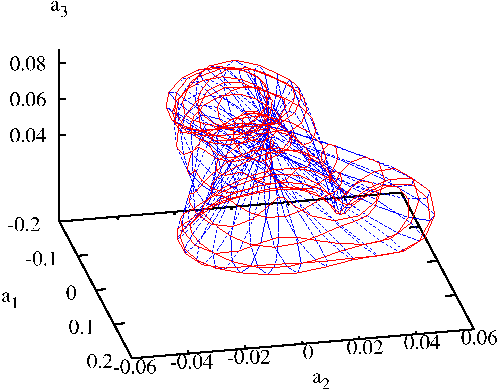
\includegraphics[width=1.20\textwidth]{2840GOt135M1} %{2830GO7}
%  \caption{\label{fig:2830GO6}
    %\label{fig:M1groupOrb}
%
and the phase velocity $\dot{\gSpace}(\sspRSing)$ in \refeq{reconstrEq}
diverges.  For points more distant the group orbits have more than one
intersection with the \slice\ hyperplane. It is clear what the trouble
with any single \slice\ hyperplane is: our slice condition and \slice s
are linear.

The physical task is to, for a given dynamical flow, pick a set of
qualitatively distinct {\template s} (for example, one typical of 2-roll
states, one for 4-roll states, and so on) whose \slice s  are locally
transverse to open sets of nearby orbits, and which together provide a
good global atlas of $\pS/\Group$. Each \slice\ $\pS{}^{(j)}$, provides a
local chart at $\slicep{}^{(j)}$ for a neighborhood of an important,
qualitatively distinct class of solutions. Together they `Voronoi'
tessellate  the curved manifold in which the symmetry-reduced strange
attractor is embedded by a finite set of hyperplane tiles.
For further discussion, see \refappe{appe:slice}.



\section{How to slice a pipe}
\label{s:algorithm}
% former siminos/atlas/algorithm.tex

\subsection{Rotation into the \slice}

As long as the
norm is discretization independent, the \slice\ condition \refeq{eq:slcond}
is independent of the numerical representation $\ssp$
of the flow $\vec{u}$, be
it finite difference, spectral, and so on.
The slice condition is solved for $\shift$
every few time steps using Newton's method,
where a good initial guess for $\shift(\zeit)$ is obtained from
the previous value and $\dot{\shift}(\zeit)$.

When ${\sspRed}(\zeit)$ is close to ${\slicep}$ the function $f(\shift)$
has only one root.
When ${\ssp}(\zeit)$ is far from ${\slicep}$, however, $f(\shift)$
may have many roots, pairs of which may disappear with time.
This would lead
to a discontinuity in $\shift(\zeit)$.  As explained in
\refsect{s:chartingslice}, o avoid this, a global
atlas has to be pieced together from local \slice\ charts, fixed by
a well-chosen set of
\template s $\slicep{}^{(j)}$ .
Shifts $\shift_j(\zeit)$ are tracked for each local \slice\ chart $\pS{}^{(j)}$,
such that the next $\shift_{j+1}(\zeit)$ is selected at intersection with
$\pS{}^{(j+1)}$
to minimise $\Norm{{\ssp}-{\ssp_i}}$.


\subsection{Dynamically important solutions and Newton's method}
\label{s:reqva}

These solutions evolve in time along their
group orbit, generated by $\LieEl(0,\shift)$. They therefore satisfy the
\slice\ condition \refeq{eq:slcond} for $\shift(\zeit)=c\zeit +const$.
%%
When the \mslices\ is applied, should a trajectory
$\ssp(\zeit)$ approach a {\reqv} in our numerical simulation,
its phase velocity is easily determined by $\shift(\zeit)$.

The way in which the \mslices\ enables to find initial
guesses for $(\vec{u}(0),\period{},\shift)$, is the main differences
between this study and the previous ones.

Here we take as initial guesses samples of nearly recurrent velocity
fields generated by long-time simulations of turbulent dynamics
\citep{pchaot,CviGib10}. The intent is to find the {\em dynamically most
important} solutions, by sampling the turbulent flow's natural measure.
In practice, sufficiently good full \statesp\ initial guesses for
$(\vec{u}(0),\period{},\shift)$ would be almost impossible to find.
Checking correlations between $\vec{u}(\zeit)$ and
$\LieEl(0,\shift)\,\vec{u}(\zeit-\period{})$ for each $\period{}$, and
more problematically, for all possible shifts $(\phi,\shift)$, is an
unrealistic task. The \mslices, however, enables us determine close
recurrences  from the symmetry-reduced time series, and locates the
dynamically most important solutions, \ie, those trajectories that are
most likely to be observed in a long-time turbulent simulation. The \rpo
s are reduced to \po s, whose unstable manifolds are much easier to track
in the \reducedsp. The \rpo\ shift $\shift$ is given by the
reconstruction equation, \refeq{reconstrEq}, or, in practice, by phase
shift $\shift(\period{})-\shift(0)$ accumulated by the intermediate
Newton steps that keep the orbit within the slice.

With a good initial guess for $(\vec{u}(0),\period{},\shift)$, such a
system can be solved using a Newton scheme.  Two conditions in addition
to \refeq{eq:fRPO} are need to be enforced: the Newton update should have no
component along the group orbit, $\braket{\vec{\delta
u}}{\groupTan(\vec{u})}=0$, and no component tangent to trajectory,
$\braket{\vec{\delta u}}{\dot{\vec{u}}}=0$.

\section{Sliced pipe}
\label{s:slicedWurst}
% former siminos/atlas/reqva.tex

%\subsection{Pipe flow \reqva\ sliced}
%\label{s:eqbSols}

%\begin{figure}
%  \centering
%  \includegraphics[width=0.6\textwidth]{1611M1PROJ_loc2} %../figs/M1PROJ_loc2.eps}
%  \caption{ \label{fig:M1loc2}
%  (color online)
%    Projection of the dynamics local to the N2\_M1 state.
%    The {\reqv} has been reduced to the central
%    \eqv\ within the \slice.  The local spiral of unstable trajectories
%    is now clearly revealed, the N2\_M1 state having only a single
%    complex unstable eigenvalue within its symmetry class.
%    $\sspRed_i(\zeit) = \langle \be_i | \sspRed(\zeit)-\sspRed_\mathrm{N2\_M1}\rangle$,
%    where $\be_1$ and $\be_2$ are unit vectors along
%    real and imaginary components of the unstable eigenvector.
%  }
%\end{figure}
To project on to the two dimensions of the page,
deviations from the M1 state have been projected against the
real and imaginary components of the M1 complex eigenvectors
$\vec{e}_1$ and $\vec{e}_2$ respectively.
\refFig{fig:M1loc2} shows the local spiral of trajectories
initially perturbed from M1 (blue circle).

For these symmetry reductions, a single \template\
$\slicep = \ssp_{\mathrm{M1}}(0)$ sufficed.
Without restriction of dynamics to the $\Omega_2$-invariant subspace,
trajectories stray much further from M1, so in order to track
such trajectories, all {\reqva}
states were deployed as templates,  $\slicep{}^{(j)}$, $j=1,2,\cdots,6$.
Switching from one local slice to the next nearest one keeps the phase
velocity \refeq{reconstrEq} finite (see \reffig{fig:thetadot}) and
enables tracking of turbulent trajectories in the \reducedsp.


\subsection{Pipe flow \rpo s sliced}
\label{s:rpos}
% former siminos/atlas/rpos.tex

 Without symmetry reduction, the detection
of the nearest recurrence of a state near a previous state, earlier on the
the same trajectory,
would require the calculating the minimum over all possible shifts.
Within the symmetry-\reducedsp\ the determination of recurrences is simple,
as the slices are constructed by requiring that the slice points are
the minimum distance points between the group orbits of the two states.
\refFig{fig:NormDiff} shows the signal for detecting a nearby \rpo\
that shadows the turbulent trajectory.  States from the indicated minimum,
along with the stream-wise shift between start and end of the candidate trajectory,
determined from $\shift(\zeit)-\shift(\zeit-\Delta t)$,
were passed to the Newton--Krylov code.


\section{Conclusion and perspectives}
\label{s:concl}
% former siminos/atlas/concl.tex

As a turbulent flow evolves, every so often we catch a glimpse of a
familiar structure. For any finite spatial resolution, the flow
follows for a finite time a coherent structure belonging to an
alphabet of admissible fluid states, represented here by a set of \reqv\
and \rpo\ solutions of \NS. These are not the `modes' of the fluid; {they
do not provide a decomposition of the flow into a sum of components at
different wavelengths, or a basis for low-dimensional
modeling.} Each such solution spans the whole range of physical scales of
the turbulent fluid, from the outer wall-to-wall scale, down to the
viscous dissipation scale. Numerical computations require sufficient
resolution to cover all of these scales, so no {global} dimension
reduction is likely. The role of invariant solutions of \NS\ is, instead,
to partition the $\infty$-dimensional \statesp\ into a finite set of
neighborhoods visited by a typical long-time turbulent fluid state.

Motivated by the recent observations of \recurrStr s in experimental and
numerical turbulent flows, we initiated here an exploration of the
hierarchy of \reqva\ and \rpo s of fully-resolved transitionally
turbulent pipe flow in order to describe its spatio-temporally chaotic
dynamics. The $3D$ fluid states captured by the short pipe invariant
solutions and their unstable manifolds are strikingly similar to states
observed both in experiments and in numerical simulations of longer pipes
\citep{science04}, while the turbulent dynamics visualized in \statesp\
appears pieced together from close visitations to \cohStr s connected by
transient interludes.

For pipe flow \reqva\ and \rpo s embody a vision of turbulence as a
repertoire of recurrent spatio-temporal coherent structures explored by
turbulent dynamics. Given a set of invariant solutions, the next
step is to understand how the dynamics interconnects the neighborhoods of
the invariant solutions discovered so far.
        %
Currently, a taxonomy of these myriad states eludes us, but emboldened by
successes in applying periodic orbit theory to the simpler \KS\ problem
\citep{Christiansen97,lanCvit07,SCD07}, we are optimistic.

The reader might rightfully wonder what the short pipe periodic cells
studied here and in \pCf\ have to do with physical,
wall-bounded shear flows in general, with large aspect ratios and
physical boundary conditions. Indeed, the outstanding issue
that must be addressed in future work is the small-aspect cell
periodicities imposed for computational efficiency. In case of the pipe
flow, most computations of invariant solutions have focused on
stream-wise periodic cells barely long enough to allow for sustained
turbulence. Such small cells introduce dynamical artifacts such as lack
of structural stability and cell-size dependence of the sustained
turbulence states.

The main message of this paper is that if a problem has a continuous
symmetry, the symmetry \emph{must} be used to simplify it. Ignore it at
your own peril, as has been done so far in \KS\ \citep{Christiansen97}
and \pCf\ \citep{GHCW07}; the invariant solutions found by restricting
searches to the discrete-symmetry invariant subspaces have little if
anything to do with the full \statesp\ explored by turbulence, not more
than the \eqv\ points of the Lorenz equation have to do with its strange
attractor. Symmetry reduction by \mslices\ is numerically efficient.
Coupled with our \statesp\ visualizations allows for explorations of
high-dimensional flows that hitherto were unthinkable. Symmetry reduction
is here achieved, and now all pipe flow solutions can be plotted
together, as one happy family: all points equivalent by symmetries are
represented by a single point, families of solutions are mapped to a
single solution, \reqva\ become \eqva, and \rpo s become \po s. Without
symmetry reduction, no full understanding of pipe and plane \pCf s is
possible.
    %
    \PC{2011-10-18 incorporate this paragraph:``
Note also that the rotation of a fluid flow into a \slice\ {\em is not}
an average over the 3D pipe azimuthal angle, it is the full snapshot of
the flow embedded in the $\infty$-dimensional \statesp. Symmetry
reduction is not a dimensional-reduction scheme, or flow modeling by
fewer degrees of freedom: the \reducedsp\ is also $\infty$-dimensional
and no information is lost, one can go freely between solutions in the
full and reduced \statesp s by integrating the associated
\emph{reconstruction equations}.
''}

\begin{acknowledgments}
We are indebted to
M.~Avila,
D.~Barkley,
R.~L.~Davidchack,
S.~Froehlich,
E.~Siminos
L.~S.~Tuckerman,
and
A.~P.~Willis
% D.~Viswanath
for inspiring discussions.
P.~C.\ thanks G.~Robinson,~Jr.\ for support, and
Max-Planck-Institut f\"ur Dynamik und Selbstorganisation,
G\"ottingen for hospitality.
P.~C.\ was partly supported by NSF grant DMS-0807574
and
2009 Forschungspreis der Alexander von Humboldt-Stiftung.
\end{acknowledgments}

\appendix

\section{Global atlas}
\label{appe:slice}
% Predrag 2011-10-15: transferred here text from slice.tex

A hyperplane captures faithfully neighboring group orbits until,
for a point not so close
\[
\braket{\groupTan(\sspRSing)}{\sliceTan{}}= 0
\,.
\]
%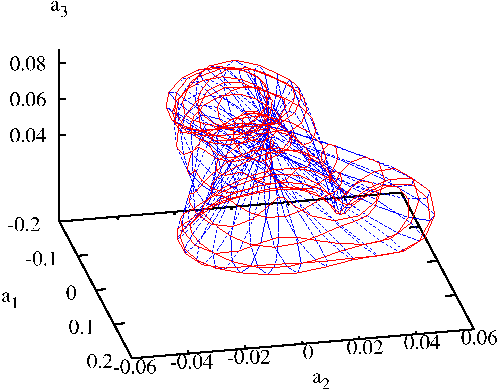
\includegraphics[width=1.20\textwidth]{2840GOt135M1} %{2830GO7}
%  \caption{\label{fig:2830GO6}
    %\label{fig:M1groupOrb}
%
The phase velocity $\dot{\gSpace}(\sspRSing)$ in
\refeq{reconstrEq} then diverges. Equivalently,
one can say that a \slice\ is transverse to a group orbit as long as the
curvature normal vector \refeq{eq:curv}, does not lie in the \slice,
    \PC{should I say that curvature distinguishes the minima, say it
        an appendix, or not say it at all in this paper?
    {\bf APW 111020} I can imagine the situation of the previous equation
    but have trouble imagining that of the next eqn.
    Possibly leave in appendix - see next comment.
}
\[
\braket{\groupTan(\sspSing)}{\sliceTan{}}
 =
-\braket{\sspSing}{\Lg^2\slicep}
 =
-\braket{\sspSing}{\kappa(\slicep) \, {n}(\slicep)}
 = 0
\,.
\]
This is also a linear condition, and it defines a hyperplane of points
\sspSing\ normal to  the quadratic Casimir-weighted curvature vector
$\kappa(\slicep) \, {n}(\slicep)$, such that from the {\template} vantage
point their group orbits are not transverse, but locally `horizontal.'
%$(d\!-\!2)$\dmn\
{\Sset} $S$ is the locus of inflection points, a hyperplane through which
curvature of the distance function changes sign: set of all points
$\sspRSing$ which are both in the {\slice}, and whose group tangent
$\groupTan(\sspRSing)$ is also in the  {\slice},
    \PC{add Froehlich figure of {\Sset} $S$?}
    % 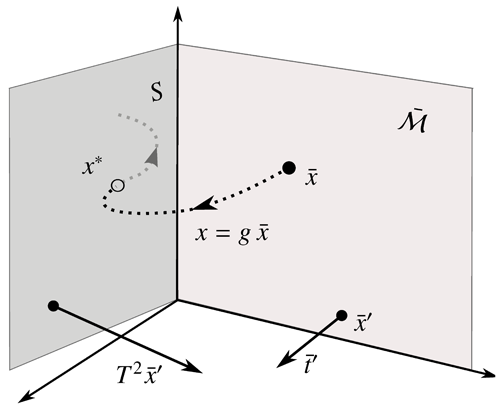
\includegraphics[width=0.80\textwidth]{inflectHype.png}
\beq
\braket{\sspRSing}{\sliceTan{}} \,=\, 0
    \,, \mbox{ and }
\braket{\groupTan(\sspRSing)}{\sliceTan{}}
 \,=\,
-\braket{\sspRSing}{\kappa(\slicep) \, {n}(\slicep)}
 =0
\,.
\label{sliceSingl0}
\eeq
A hyperplane segment of a \slice\ is good only up to the \sset. However,
the divergence in phase velocity \refeq{reconstrEq} is an artifact of
the symmetry reduction by tangent hyperplanes, and thus an avoidable
nuisance.
\APW{111020 OK... starting to think a (very streamlined) note ought
to be in the main text - e.g. first 2 sentences of app B and the next
sentence appear to be sufficient.
\\
{\bf Predrag 111020}
I've written this so many times that I am blind to its obvious faults.
Can you do the next rewrite of the atlas (both main text and the appendix)
and I or Marc will take it from there...
}

Locally, our initial \slice\ chart $\pSRed{}^{(1)}$ is a ($d\!-\!1$)\dmn\ hyperplane.
If
we pick another {\template} point $\slicep{}^{(2)}$, it comes along with
its own \slice\ hyperplane $\pSRed{}^{(2)}$.
Any neighboring pair of
$(d\!-\!1)$\dmn\ local \slice\ hyperplanes intersects in a `ridge',
% (`boundary,' `edge'),
a $(d\!-\!2)$\dmn\ hyperplane, easy to compute.

Thus, in order to chart the \statesp\ of a turbulent flow, a set
of local \slice\ hyperplanes is needed to capture all of the asymptotic
dynamics. The choice of local \slice s should reflect the dynamically
dominant patterns seen in the solutions of nonlinear PDEs. We construct a
global atlas of the dimensionally \reducedsp\ $\pSRed = \pS/\Group$ by
deploying local linear \slice s  $\pS{}^{(j)}$ across neighborhoods of
the qualitatively most important \template\ {\cohStr s}
$\slicep{}^{(j)}$. For example, in reducing turbulent trajectories of
\refsect{s:rpos}, we use a set of \reqva\ as our templates, see
\reffig{fig:thetadot}. This is the periodic-orbit implementation of the
idea of {\statesp\ tessellation}.
% 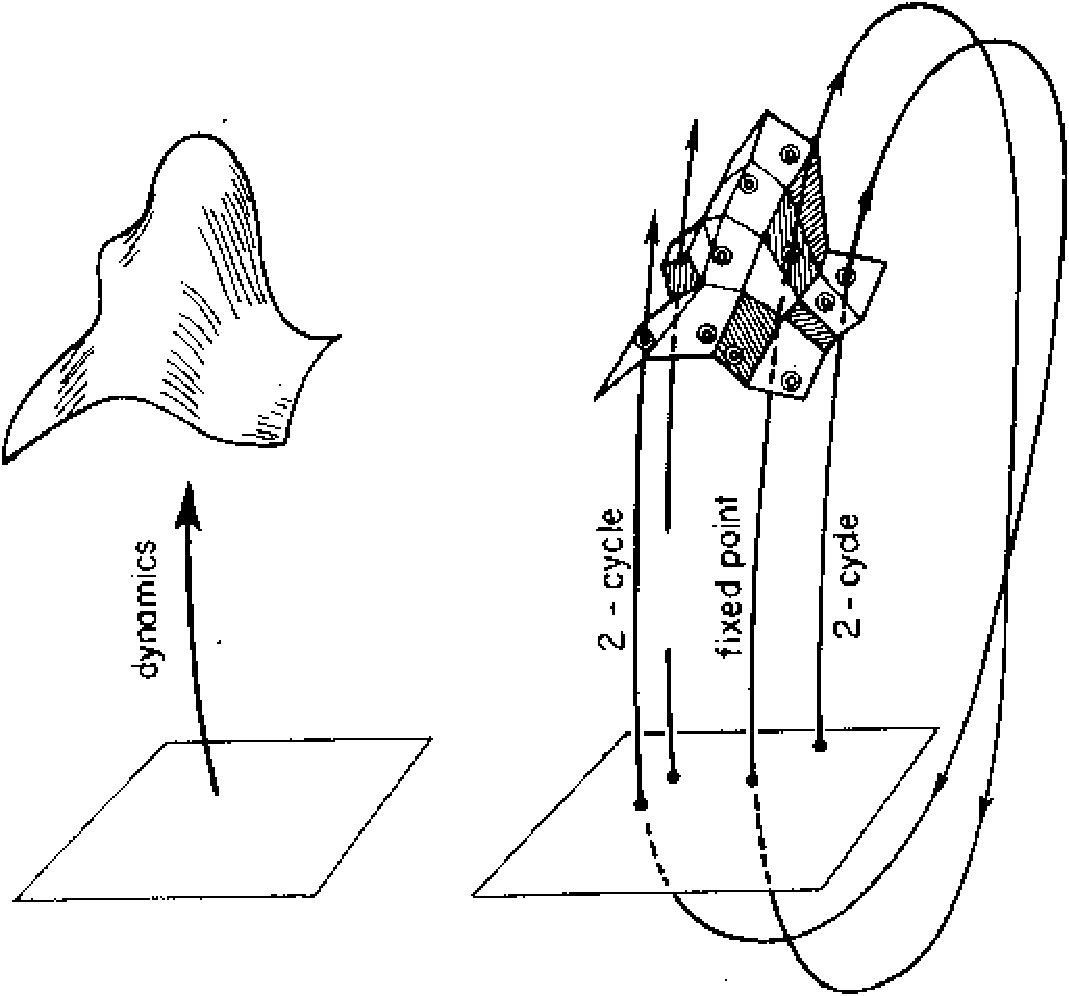
\includegraphics[width=0.60\textwidth]{f_1_08_1}
    \PC{please, as few \template s as possible in \reffig{fig:thetadot}.
And there should be no jumps in $\dot{\gSpace}(\sspRSing)$, none at all.
We just need to make sure that the ridges between the templates are
sufficiently close to each the templates, so that the {\sset s} are
excluded. Once templates are picked, the rest is geometry of hyperplanes
(NOTHING to do with dynamics, only with the group theory) so checking
whether the inflection hyperplane is on the far side of the tile edge
(ridge between two \slice s) is a linear computation, to be undertaken
independently of dynamics.

If the jumps are genuine and non-removable by refinements of slice
charts, that's a big deal. It indicates that the generic turbulent orbit
makes arbitrarily close passages to invariant subspace(s), and that is
physical, not a chart artifact. Are there physical states that are like
Hagen \eqv, but stream-wise deformed, \ie\ is there a nontrivial subspace
invariant under the whole symmetry $\Group = \On{2}_\theta \times
\SOn{2}_z$?
}

    \PC{merge with the paragraph above}
The physical task is to, for a given dynamical flow, pick a set of
qualitatively distinct {\template s} whose \slice s  are locally
transverse to an open set of nearby orbits. Each \slice\ $\pS{}^{(j)}$,
provides a local chart at $\slicep{}^{(j)}$ for a neighborhood of an
important, qualitatively distinct class of solutions (2-rolls states,
3-rolls states, \etc). Together they `Voronoi' tessellate  the curved
manifold in which the symmetry-reduced strange attractor is embedded by a
finite set of hyperplane tiles. We have no advice on how to
systematically pick the individual templates, other than that the
associated \slice\ tiles should be sufficiently small to exclude
group-orbit tangencies, \ie, stop before crossing their inflection
hyperplanes \refeq{sliceSingl0}.


\bibliographystyle{jfm}
\bibliography{../bibtex/siminos}

\PublicPrivate{}{
\newpage
\input flotsam
\newpage
\section{Daily blog, point by point}
\input ../blog/atlas
%\input ../blog/flotsam
    } % end \PublicPrivate

\end{document}
